
%%%%%%%%%%%%%%%%%%%%%%%%%%%%%%%%%%%%%%%%%%%%%%%%%%%%%%%%%%%%%%%%%%%%%%%
%%%%%%%%%%%%%%%%%%%%%%%%%%%%%%%%%%%%%%%%%%%%%%%%%%%%%%%%%%%%%%%%%%%%%%% 
%%%%%%%%%%%       								 Preamble				         	                                                        %%%%%%%%%% 
%%%%%%%%%%%%%%%%%%%%%%%%%%%%%%%%%%%%%%%%%%%%%%%%%%%%%%%%%%%%%%%%%%%%%%% 
%%%%%%%%%%%%%%%%%%%%%%%%%%%%%%%%%%%%%%%%%%%%%%%%%%%%%%%%%%%%%%%%%%%%%%% 
\documentclass[10pt]{beamer}
\usepackage{setspace}
\usepackage{color}
\usepackage{amsmath,lmodern}
\usepackage{hyperref}
\usepackage{graphicx}
\usepackage{multirow}
\usepackage{tikz}
\usetikzlibrary{fit,shapes.misc}
\usepackage{pdflscape}
\usepackage{amsmath}
\usepackage{lscape}
\usepackage{multirow}
\usepackage{enumerate}
\usepackage{epstopdf}
\usepackage{pdfpages}
\usepackage{appendixnumberbeamer}
\usepackage{color,soul}
\usepackage{grffile}
\usepackage{float}
\usepackage{relsize}
\usepackage{tcolorbox}
\newcounter{nodemarkers}
\usepackage{tikz}
\newcommand{\toplinesmall}{%
  \tikz[remember picture,overlay] {%
    \draw[blue,thick] ([yshift=-1cm, xshift=.9cm]current page.north west)
             -- ([yshift=-1cm,xshift=3.6cm]current page.north west);}}
             
\newcommand{\toplinemedium}{%
  \tikz[remember picture,overlay] {%
    \draw[blue,thick] ([yshift=-1cm, xshift=.9cm]current page.north west)
             -- ([yshift=-1cm,xshift=6.2cm]current page.north west);}}
 
 \newcommand{\toplinelarge}{%
  \tikz[remember picture,overlay] {%
    \draw[blue,thick] ([yshift=-1cm, xshift=.9cm]current page.north west)
             -- ([yshift=-1cm,xshift=8.9cm]current page.north west);}}           
             
 \newcommand{\toplinexlarge}{%
  \tikz[remember picture,overlay] {%
    \draw[blue,thick] ([yshift=-1cm, xshift=.9cm]current page.north west)
             -- ([yshift=-1cm,xshift=12cm]current page.north west);}}                       
             
\setbeamertemplate{footline}
{
  \leavevmode%
  \hbox{%
  \begin{beamercolorbox}[wd=.333333\paperwidth,ht=2.25ex,dp=1ex,center]{author in head/foot}%
    \usebeamerfont{author in head/foot}{\textcolor{blue}{ECON311}}
  \end{beamercolorbox}%
  \begin{beamercolorbox}[wd=.333333\paperwidth,ht=2.25ex,dp=1ex,center]{title in head/foot}%
    \usebeamerfont{title in head/foot}{\textcolor{blue}{Winter 2026}}
  \end{beamercolorbox}%
  \begin{beamercolorbox}[wd=.333333\paperwidth,ht=2.25ex,dp=1ex,right]{date in head/foot}%
    \usebeamerfont{date in head/foot}{\textcolor{blue}{Lecture 8 \: \: \: \: \: \: \: }
    \insertframenumber{} / \inserttotalframenumber\hspace*{2ex}} 
  \end{beamercolorbox}}%
  \vskip0pt%
}
\newtheorem{proposition}[theorem]{Proposition}

\newcommand\marktopleft[1]{%
    \tikz[overlay,remember picture] 
        \node (marker-#1-a) at (-0.2,1.2ex) {};%
}
\newcommand\markbottomright[1]{%
    \tikz[overlay,remember picture] 
        \node (marker-#1-b) at (0.16,-1ex) {};%
    \tikz[overlay,remember picture,thick,inner sep=4pt]
        \node[draw,rectangle,rounded corners, blue, fit=(marker-#1-a.center) (marker-#1-b.center)] {};%
}

\setbeamertemplate{caption}{\raggedright\insertcaption\par}
\setbeamertemplate{itemize items}[ball]
\setbeamertemplate{itemize subitem}[triangle]
\setbeamertemplate{itemize subsubitem}[triangle]
\tcbset{colframe=white,colback=white,nobeforeafter}
\beamertemplatenavigationsymbolsempty
\addtobeamertemplate{frametitle}{\vspace*{0.19cm}}{\vspace*{0cm}}


%%%%%%%%%%%%%%%%%%%%%%%%%%%%%%%%%%%%%%%%%%%%%%%%%%%%%%%%%%%%%%%%%%%%%%%
%%%%%%%%%%%%%%%%%%%%%%%%%%%%%%%%%%%%%%%%%%%%%%%%%%%%%%%%%%%%%%%%%%%%%%% 
%%%%%%%%%  									    Define Title									                                       %%%%%%%%%
%%%%%%%%%%%%%%%%%%%%%%%%%%%%%%%%%%%%%%%%%%%%%%%%%%%%%%%%%%%%%%%%%%%%%%%
%%%%%%%%%%%%%%%%%%%%%%%%%%%%%%%%%%%%%%%%%%%%%%%%%%%%%%%%%%%%%%%%%%%%%%% 
\title{ECON 311} 
\author{Lecture 8: Solow Growth Model, part III}
\date{}
\AtBeginSection[]
{
 \begin{frame}<beamer>
 \tableofcontents[currentsection]
 \end{frame}
}
%%%%%%%%%%%%%%%%%%%%%%%%%%%%%%%%%%%%%%%%%%%%%%%%%%%%%%%%%%%%%%%%%%%%%%%
%%%%%%%%%%%%%%%%%%%%%%%%%%%%%%%%%%%%%%%%%%%%%%%%%%%%%%%%%%%%%%%%%%%%%%% 
%%%%%%%% 						     				Document								                                                %%%%%%%%
%%%%%%%%%%%%%%%%%%%%%%%%%%%%%%%%%%%%%%%%%%%%%%%%%%%%%%%%%%%%%%%%%%%%%%%
%%%%%%%%%%%%%%%%%%%%%%%%%%%%%%%%%%%%%%%%%%%%%%%%%%%%%%%%%%%%%%%%%%%%%%% 
\begin{document}
\setbeamercovered{transparent}

\begin{frame}
\maketitle
\end{frame}

%%%%%%%%%%%%%%%%%%%%%%%%%%%%%%%%%%%%%%%%%%%%%%%%%%%%%%%%%%%%%%%%%%%%%%%
%%%%%%%%%%%%%%%%%%%%%%%%%%%%%%%%%%%%%%%%%%%%%%%%%%%%%%%%%%%%%%%%%%%%%%% 
%%%%%%%% 						     				Introduction	             		                                		  %%%%%%%%
%%%%%%%%%%%%%%%%%%%%%%%%%%%%%%%%%%%%%%%%%%%%%%%%%%%%%%%%%%%%%%%%%%%%%%%
%%%%%%%%%%%%%%%%%%%%%%%%%%%%%%%%%%%%%%%%%%%%%%%%%%%%%%%%%%%%%%%%%%%%%%% 


\begin{frame}
\frametitle{\: \: \: Solving for Equilibrium}
\toplinelarge
\begin{itemize}
\item For any $t$, the aggregate economy in the Solow Model is characterized by five equations and five unknowns ($K_t, L_t, I_t, C_t, Y_t$):
\begin{eqnarray*}
\begin{array}{ll}
\Delta K_{t+1}=\overline{s} F(K_t,L_t)-\overline{d}K_t & (\text{law of motion}) \\[1.4ex]
Y_t=\overline{A}K_t^{\frac{1}{3}}L_t^{\frac{2}{3}}& (\text{production function}) \\[1.4ex]
C_t+I_t=Y_t & (\text{resource constraint}) \\[1.4ex]
L_t=\overline{L}& (\text{labour force}) \\[1.4ex]
I_t=\overline{s} Y_t  & (\text{allocation of resources}) 
\end{array}
\end{eqnarray*}
\item For an initial level of capital, $K_0$, we can solve for the endogeneous variables in any time period.
\begin{itemize}
\vspace{.11in} 
\item Instead of solving the model for any time period, which requires a lot of algebra, we will only solve analitically for the steady state (ss) and provide graphical interpretation for other time periods.
\end{itemize}
\end{itemize}  
\end{frame} 

\begin{frame}
\frametitle{\: \: \: Output and Consumption per capita}
\toplinexlarge
\begin{itemize}
\item An important variable in the Solow Model is the level of consumption at time $t$, which can be written as:
\begin{eqnarray*}
C_t=(1-\overline{s})Y_t
\end{eqnarray*}
\end{itemize}
\begin{figure}
\centering
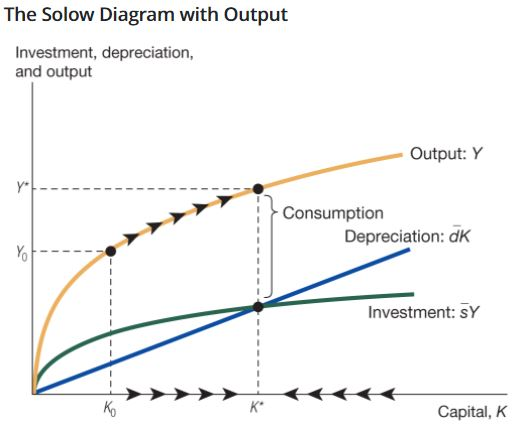
\includegraphics[scale=.49]{Solow_output}
\end{figure}
\end{frame}

\begin{frame}
\frametitle{\: \: \: Output and Consumption per capita}
\toplinexlarge
\begin{itemize}
\item The resource constraint formalizes the trade-off an economy faces:
\begin{itemize}
\vspace{.11in} 
\item In order to grow faster and achieve higher production and higher consumption in the long run, initial consumption must be lower.
\end{itemize}
\vspace{.11in} 
\item We can see this point in our example of the Canadian and Argentine economies:
\begin{eqnarray*}
\begin{array}{ll}
t=0 & c_0^{ARG}=(1-\overline{s}_{ARG}) \overline{A}\left(\frac{K_0}{\overline{L}}\right)^{\frac{1}{3}} > (1-\overline{s}_{CAN}) \overline{A} \left(\frac{K_0}{\overline{L}}\right)^{\frac{1}{3}}=c_0^{CAN} \\[3ex]
\end{array}
\end{eqnarray*}
\end{itemize}
\end{frame}

\begin{frame}
\frametitle{\: \: \: Output and Consumption per capita}
\toplinexlarge
\begin{figure}
\centering
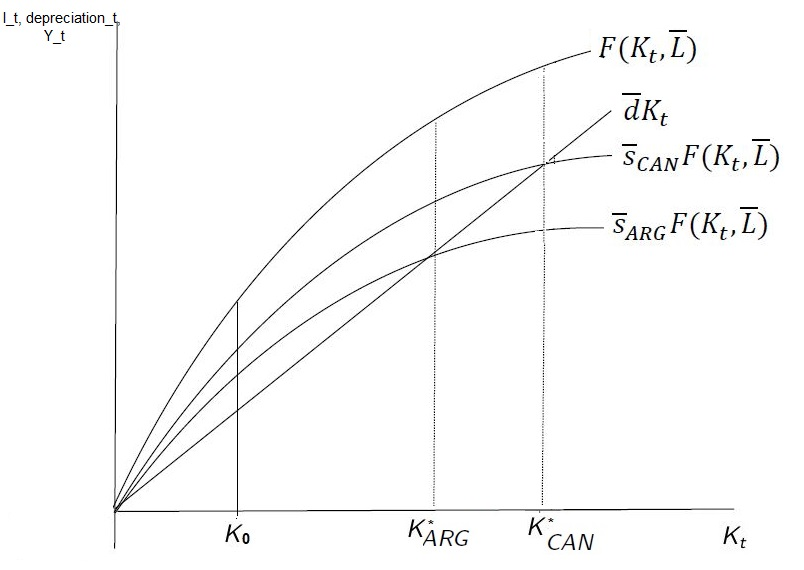
\includegraphics[scale=.48]{Solow_consumption}
\end{figure}
\end{frame}


\begin{frame}
\frametitle{\: \: \: Solving for Steady State}
\toplinexlarge
\begin{itemize}
\item To solve for the steady state equilibrium, we can reduce the equilibrium conditions to three equations and three unknowns:
\footnotesize 
\begin{eqnarray*}
\begin{array}{lllll}
\Delta K_{t+1}=0 & \Rightarrow & K^*=\overline{L}\left(\frac{\overline{s}\overline{A}}{\overline{d}}\right)^{\frac{3}{2}} & , & k^*=\left(\frac{\overline{s}\overline{A}}{\overline{d}}\right)^{\frac{3}{2}}\\[3ex]
Y^*=\overline{A}\left(K^*\right)^{\frac{1}{3}}\left(\overline{L}\right)^{\frac{2}{3}} &\Rightarrow & Y^*=\overline{L} \: \: \: \: \overline{A}^{\frac{3}{2}}\left(\frac{\overline{s}}{\overline{d}}\right)^{\frac{1}{2}} &, &  y^*=\overline{A}^{\frac{3}{2}}\left(\frac{\overline{s}}{\overline{d}}\right)^{\frac{1}{2}} \\[3ex]
C^*=(1-\overline{s})Y^* & \Rightarrow & C^*=(1-\overline{s}) \overline{L} \: \: \: \: \overline{A}^{\frac{3}{2}}\left(\frac{\overline{s}}{\overline{d}}\right)^{\frac{1}{2}}& , &  c^*=(1-\overline{s}) \overline{A}^{\frac{3}{2}}\left(\frac{\overline{s}}{\overline{d}}\right)^{\frac{1}{2}}
\end{array}
\end{eqnarray*}
\normalsize
\item We will also study how the system behaves out of the steady state without solving for endogeneous variables.
\begin{itemize}
\vspace{.11in} 
\item This is important to understand differences in growth rates.
\end{itemize}
\end{itemize}   
\end{frame}

\begin{frame}
\frametitle{\: \: \: An increase in savings rate $\overline{s}$}
\toplinexlarge
\begin{itemize}
\item Assume that the economy is in its steady-state equilibrium and in 2020, there is an increase in savings:
\end{itemize}
\begin{figure}
\centering
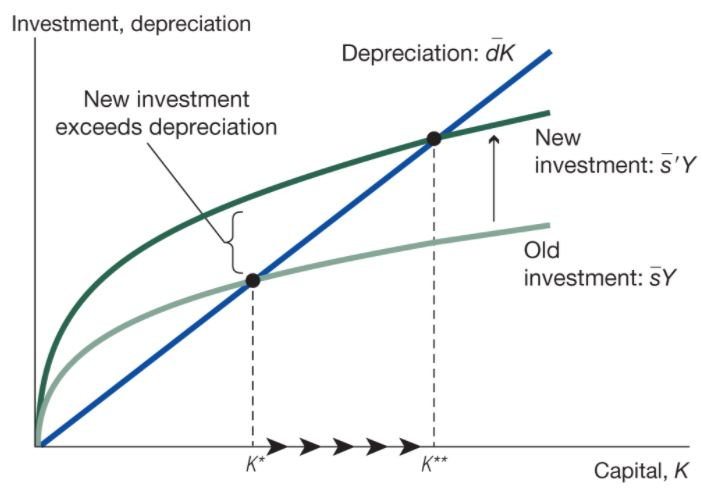
\includegraphics[scale=.5]{increase_savings}
\end{figure}
\end{frame}

\begin{frame}
\frametitle{\: \: \: An increase in savings rate $\overline{s}$}
\toplinexlarge
\begin{figure}
\centering
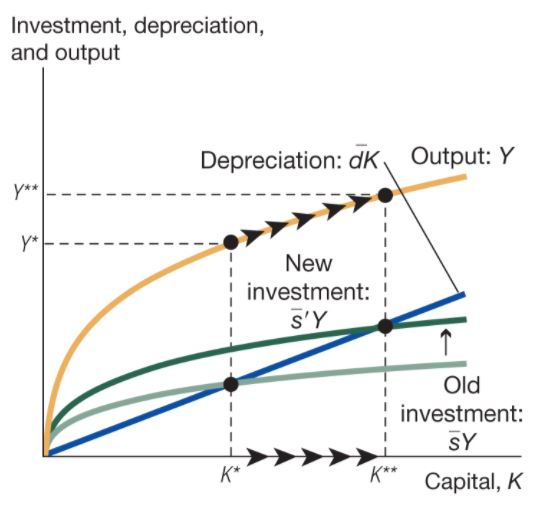
\includegraphics[scale=.65]{increase_savings_y}
\end{figure}
\end{frame}

\begin{frame}
\frametitle{\: \: \: Transition Dynamics}
\toplinexlarge
\begin{columns}
\begin{column}{0.5\linewidth}
\begin{figure}
\centering
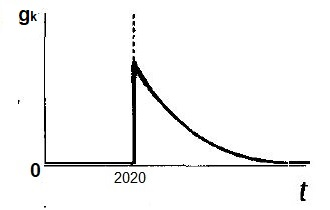
\includegraphics[scale=.54]{g_K}
\end{figure}
\end{column}
\begin{column}{0.57\linewidth}
\begin{figure}
\centering
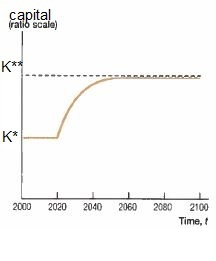
\includegraphics[scale=.5]{k_changes_savings}
\end{figure}
\end{column}
\end{columns}
\begin{columns}
\begin{column}{0.5\linewidth}
\begin{figure}
\centering
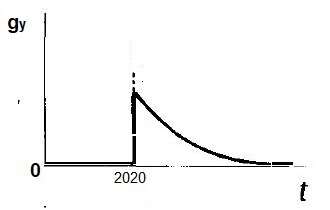
\includegraphics[scale=.54]{g_Y}
\end{figure}
\end{column}
\begin{column}{0.57\linewidth}
\begin{figure}
\centering
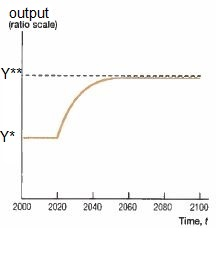
\includegraphics[scale=.5]{increase_savings_y_changes}
\end{figure}
\end{column}
\end{columns}
\end{frame}

\begin{frame}
\frametitle{\: \: \: An increase in depreciation rate $\overline{d}$}
\toplinexlarge
\begin{itemize}
\item Assume that the economy is in its steady-state equilibrium and in 2020, there is an increase in depreciation rate:
\end{itemize}
\begin{figure}
\centering
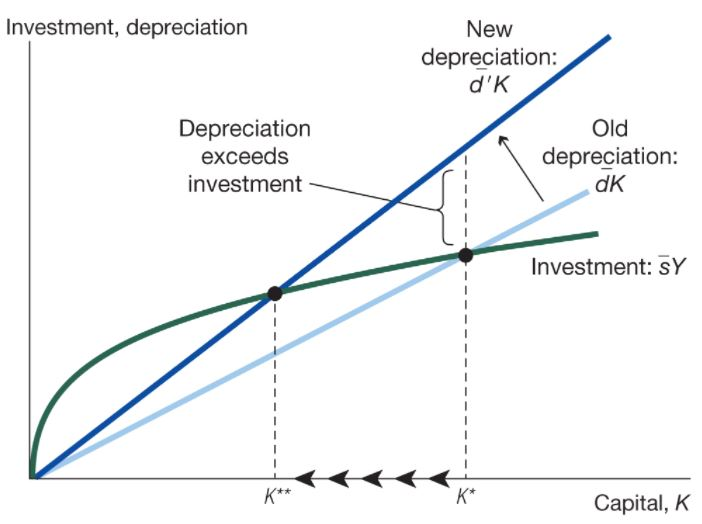
\includegraphics[scale=.5]{increase_depreciation}
\end{figure}
\end{frame}

\begin{frame}
\frametitle{\: \: \: An increase in depreciation rate $\overline{d}$}
\toplinexlarge
\begin{figure}
\centering
\includegraphics[scale=.5]{increase_depreciation_y}
\end{figure}
\end{frame}

\begin{frame}
\frametitle{\: \: \: Transition Dynamics}
\toplinelarge
\begin{columns}
\begin{column}{0.5\linewidth}
\begin{figure}
\centering
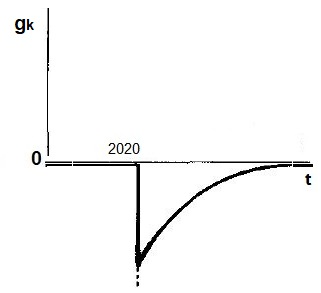
\includegraphics[scale=.45]{g_K_depreciation}
\end{figure}
\end{column}
\begin{column}{0.57\linewidth}
\begin{figure}
\centering
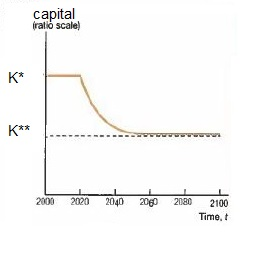
\includegraphics[scale=.5]{increase_depreciation_K_changes}
\end{figure}
\end{column}
\end{columns}
\begin{columns}
\begin{column}{0.5\linewidth}
\begin{figure}
\centering
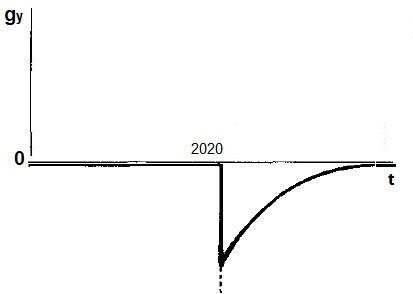
\includegraphics[scale=.34]{g_Y_depreciation}
\end{figure}
\end{column}
\begin{column}{0.57\linewidth}
\begin{figure}
\centering
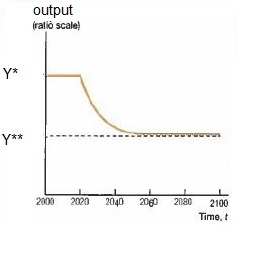
\includegraphics[scale=.5]{increase_depreciation_Y_changes}
\end{figure}
\end{column}
\end{columns}
\end{frame}





\begin{frame}
\frametitle{\: \: \: Consumption}
\toplinemedium
\begin{itemize}
\item As we showed on the ARG vs. CAN example, higher savings lead to higher GDP (per capita).
\begin{itemize}
\vspace{.11in} 
\item Households' welfare does not depend on output per capita but on consumption per capita.
\end{itemize}
\vspace{.11in} 
\item A higher level of savings, \textit{ceteris paribus}, results in ...
\begin{enumerate}
\vspace{.11in} 
\item an increase in GDP (per capita) increases consumption (per capita)
\vspace{.11in} 
\item an increase in the share of output invested decreases consumption (per capita)
\end{enumerate}
\vspace{.11in} 
\item It turns out that in the Solow Model there is a saving rate that maximizes consumption (per capita) in the steady-state
\begin{itemize}
\vspace{.11in} 
\item The amount of capital per capita maintained by this saving rate in equilibrium is called the \textit{golden-rule} level of capital.
\end{itemize} 
\end{itemize}
\end{frame}

\begin{frame}
\frametitle{\: \: \: An increase in savings rate $\overline{s}$}
\toplinexlarge
\begin{itemize}
\item Assume that the economy is in its steady-state equilibrium and there is an increase in savings:
\end{itemize}
\begin{figure}
\centering
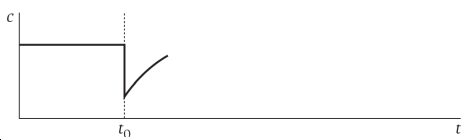
\includegraphics[scale=1.2]{consumption}
\end{figure}
\end{frame}



\begin{frame}
\frametitle{\: \: \: Consumption and Savings in the steady state}
\toplinemedium
\toplinexlarge
\begin{columns}
\begin{column}{0.5\linewidth}
\begin{figure}
\centering
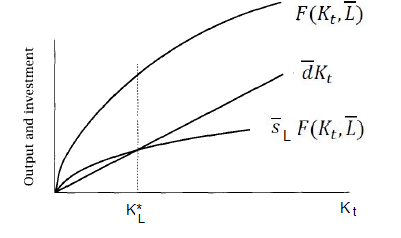
\includegraphics[scale=.5]{savings_low}
\end{figure}
\end{column}
\begin{column}{0.57\linewidth}
\begin{figure}
\centering
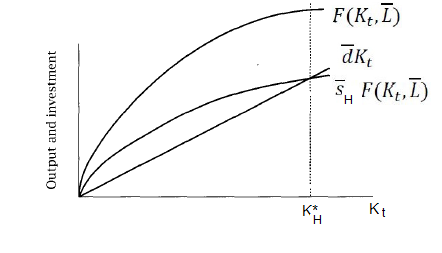
\includegraphics[scale=.5]{savings_high}
\end{figure}
\end{column}
\end{columns}
\begin{figure}
\centering
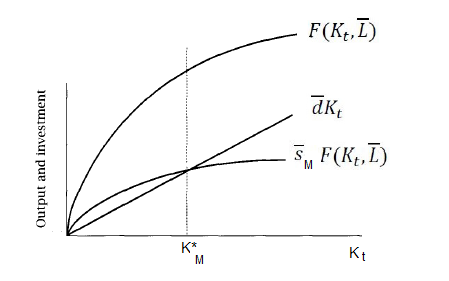
\includegraphics[scale=.5]{savings_medium}
\end{figure}
\end{frame}



\begin{frame}
\frametitle{\: \: \: Convergence with similar $y^{ss}$}
\toplinelarge
\begin{figure}
\centering
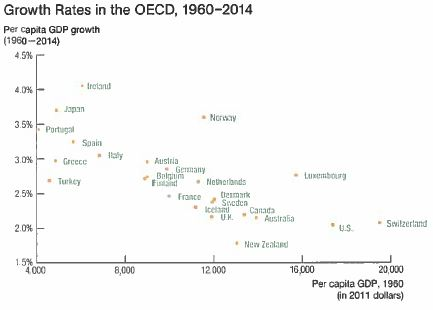
\includegraphics[scale=.75]{convergence}
\end{figure}
\end{frame}

\begin{frame}
\frametitle{\: \: \: Conclusion-- Simple Solow Model}
\toplinexlarge
\begin{itemize}
\item Provides an explanation as to why growth rates are different across countries.
\begin{itemize}
\vspace{.11in}
\item Countries have different rates of capital accumulation 
\vspace{.11in}
\item It is only useful in explaining differences among a homogeneous set of countries (with similar steady state)
\end{itemize}
\item Explicitly model the trade-off between current consumption and future growth   
\begin{itemize}
\vspace{.11in}
\item Reducing current consumption increases savings and future output
\vspace{.11in}
\item Too much savings can lead to a decrease in the steady state level of consumption
\end{itemize}
\vspace{.11in}
\item A big failure of the simple Solow Model is that ...
\begin{itemize}
\vspace{.11in}
\item  there is no economic growth in the long run.
\vspace{.11in}
\item it only provides an explanation for different $y^{ss}$ through different $k^{ss}$
\end{itemize}
\end{itemize}
\end{frame}

\end{document}


